\subsection{Flow rate in a tube with one meniscus} \label{sec:simple-flow-rate}
	At first we derive the equation for flow rate when there is one meniscus present in a tube, then we generalize the case for $n$ menisci. The flow rate of a viscous fluid through a thin tube is given by the Hagen–Poiseuille equation:
	
	\begin{equation} \label{eq:flow-rate}
		Q = \frac{\pi}{8\mu} \frac{\Delta P}{l} R^4
	\end{equation}
	
	Here, $Q$ is the volumetric flow rate in $[m^3/s]$, $\Delta P$ is the pressure difference between the ends of the tube, $\mu$ is the viscosity in $[kg/m.s]$, $l$ is the length of the tube, $R$ is the radius of the tube.
	
	\begin{figure}[H]
		\centering
		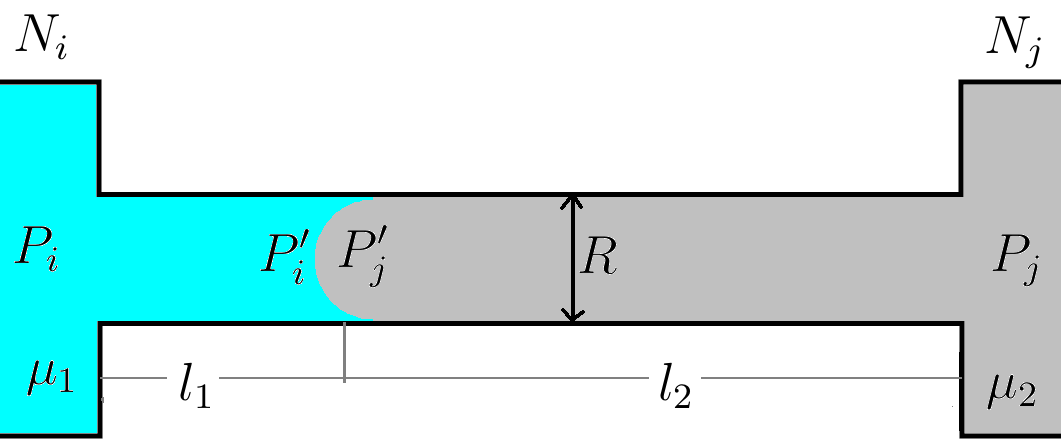
\includegraphics[width=0.6\textwidth]{fig_capillary_pressure_in_tube_1mns_blue}
		\caption{Orientation of the meniscus, the convex side contains wetting fluid while the concave side contains non-wetting fluid.}
		\label{fig_capillary_pressure_in_tube_1mns_blue}
	\end{figure}
	
	In figure \ref{fig_capillary_pressure_in_tube_1mns_blue}, node $N_{i}$ kept at a pressure of $P_{i}$, and is filled with a wetting fluid of viscosity $\mu_{1}$. Node $N_{j}$ kept at a pressure of $P_{j}$ is filled with a non-wetting fluid of viscosity $\mu_{2}$. It is evident that the pressure on the convex size or on the part of the wetting fluid is lower.
	
	\begin{equation}
		P_{i}' < P_{j}'
	\end{equation}
	
	The pressure jump is given by:
	
	\begin{equation} \label{eq:capillary_pressure_mns}
		P_{j}' - P_{i}' = \frac{2 \sigma}{R}
	\end{equation}
	
	Here, $\sigma$ is the coefficient of surface tension in $[Pa.m]$ or $[kg/s]$.
	
	Separating figure \ref{fig_capillary_pressure_in_tube_1mns_blue} into two tubes of lengths $l_{1}$ and $l_{2}$, containing fluids of viscosity ${\mu}_1$ and ${\mu}_2$. The flow rates of the tubes, from equation \ref{eq:flow-rate} are given by:
	
	\begin{equation} \label{eq:flow-rate-first}
		Q = \frac{\pi}{8{\mu}_1} \frac{P_i - P^{'}_i}{l_1} R^4
	\end{equation}
	
	\begin{equation} \label{eq:flow-rate-second}
		Q = \frac{\pi}{8{\mu}_2} \frac{P^{'}_j - P_j}{l_2} R^4
	\end{equation}
	
	Due to the law of conservation of volume, the flow rates are equal. Adding the equations \ref{eq:flow-rate-first} and \label{eq:flow-rate-second}:
	
	\begin{equation} \label{eq:flow-rate-intermediate}
		Q({\mu}_1 l_1 + {\mu}_2 l_2) = \frac{\pi}{8}R^4(P_i - P_j + P^{'}_j - P^{'}_i)
	\end{equation}
	
	Substituting the equation \ref{eq:capillary_pressure_mns} about capillary pressure,
	\begin{equation} \label{eq:flow-rate-1mns-basic-m}
		Q = \frac{\pi R^4}{8Ml} \left( \Delta P_{ij} + \frac{2\sigma}{R} \right)
	\end{equation}
	
	Here,
	\begin{equation} \label{eq:def-pressure-difference} 
		\Delta P_{ij} = P_{i} - P_{j}
	\end{equation}
	
	And $M$ is the viscosity parameter:
	\begin{equation}
		M = \sum_{k} \mu_{k} \frac{l_{k}}{l}
	\end{equation}
	Note that the viscosity parameter, remains the same for any number of menisci present in a tube.
	
\subsection{Flow rate in a tube with multiple menisci} \label{sec:multi-menisci-flow-rate}
	\begin{figure}[H]
		\centering
		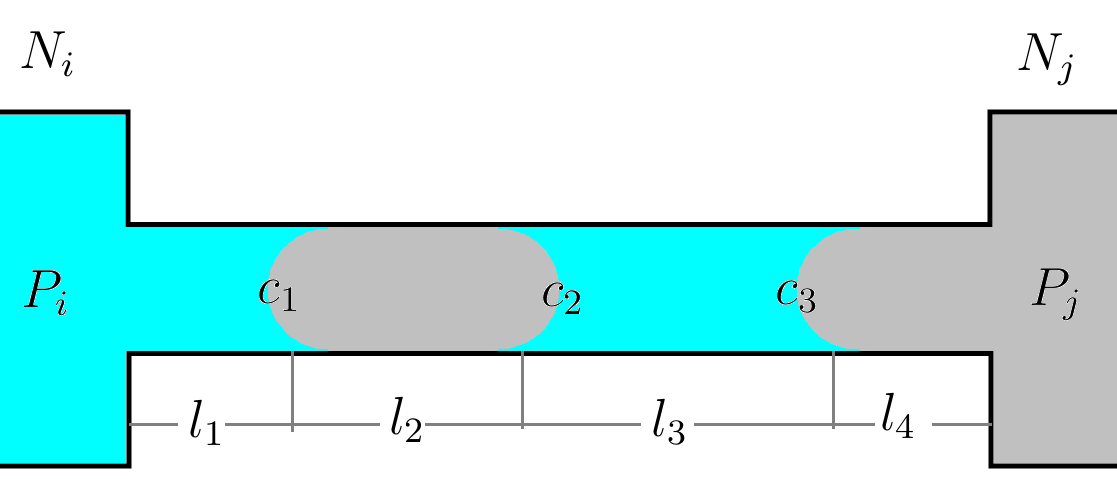
\includegraphics[width=0.6\textwidth]{fig_capillary_pressure_in_tube_3mns}
		\caption{Capillary pressure contribution, $s = 1$}
		\label{fig:capillary_pressure_in_tube_3mns}
	\end{figure}
	
	Let the capillary pressures be denoted by the following:
	\begin{equation}
		c_1 = -c_2 = c_3 = \frac{2 \sigma}{R}
	\end{equation}
	
	Then for figure \ref{fig:capillary_pressure_in_tube_3mns}, the flow rate is given by:
	
	\begin{equation}
		Q = \frac{\pi R^4}{8Ml} \left( \Delta P_{ij} + c_1 + c_2 + c_3 \right)
	\end{equation}
	
	\begin{equation}
		Q = \frac{\pi R^4}{8Ml} \left( \Delta P_{ij} + \sum_{k} c_{k} \right)
	\end{equation}
	
	Flow rate for an arbitrary number of meniscus for a cylindrical tube, is given by:
	
	\begin{equation} \label{eq:main-flow-rate-with-s}
		\boxed{Q = \frac{\pi R^4}{8Ml} \left( \Delta P_{ij} + \frac{2s \sigma}{R} \right)}
	\end{equation}
	
	Where,
	
	\begin{equation} \label{eq:sign-func-def}
		s(d, n_{mns}) = 
		\begin{dcases}
			-1,&\text{$n_{mns}$ = 1, $d$ points away from $N_{i}$}\\
			0,&\text{$n_{mns}$ = 0, 2}\\
			+1,&\text{$n_{mns}$ = 1, $d$ points towards $N_{i}$}
		\end{dcases}
	\end{equation}
	
	Here,
	\begin{itemize}
		\item $d$, the direction the convex side of the meniscus points towards
		\item $n_{mns}$, the number of meniscus in a tube
	\end{itemize}
	
	In our model, the data structure does not accommodate more than 2 meniscus in a tube, hence in the definition of $s$, $n_{mns} \le 2$. Shown that, for figure \ref{fig:capillary_pressure_in_tube_3mns}, \ref{fig:capillary_pressure_in_tube_1mns_grey}, and \ref{fig:capillary_pressure_in_tube_2mns}, $s$ is $1$, $-1$, and $0$ respectively.
	
	\begin{figure}[H]
		\centering
		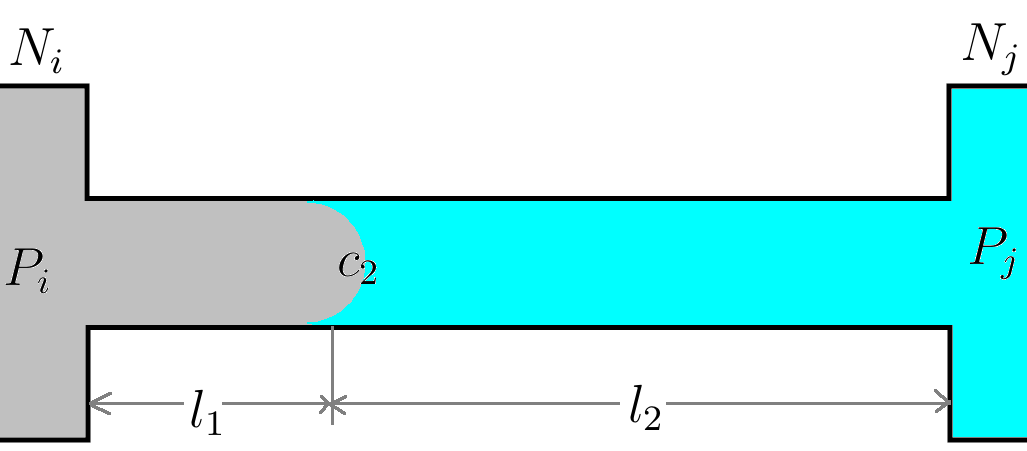
\includegraphics[width=0.6\textwidth]{fig_capillary_pressure_in_tube_1mns_grey}
		\caption{Capillary pressure contribution, $s = -1$}
		\label{fig:capillary_pressure_in_tube_1mns_grey}
	\end{figure}
	
	\begin{figure}[H]
		\centering
		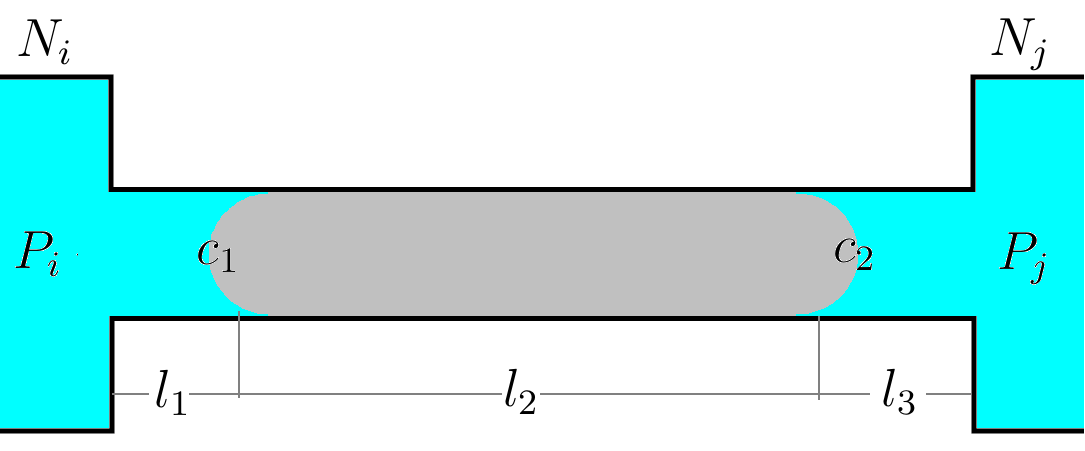
\includegraphics[width=0.6\textwidth]{fig_capillary_pressure_in_tube_2mns}
		\caption{Capillary pressure contribution, $s = 0$}
		\label{fig:capillary_pressure_in_tube_2mns}
	\end{figure}
	
\subsection{Flow rate and velocity}
	Therefore, in equation \ref{eq:flow-rate-simple-coeff}, we get:
	
	\begin{equation} \label{eq:flow-rate-aij}
		A_{ij} = \frac{\pi R_{ij}^4}{8M_{ij}l} \Delta P_{ij}
	\end{equation}
	
	\begin{equation} \label{eq:flow-rate-bij}
		B_{ij} = \frac{\pi R_{ij}^4}{8M_{ij}l} \frac{2 s_{ij} \sigma}{R_{ij}}
	\end{equation}
	
	Here, note that:
	\begin{equation}
		R_{ij} = R{ji}
	\end{equation}
	
	\begin{equation}
		M_{ij} = M{ji}
	\end{equation}
	
	\begin{equation}
		P_{ij} = -P{ji}
	\end{equation}
	
	\begin{equation}
		s_{ij} = -s{ji}
	\end{equation}
	
	When the pressures are known in each nodes, the velocity is determined by:
	\begin{equation} \label{eq:velocity-from-pressures}
		v_{ij} = \frac{Q_{ij}}{\pi R_{ij}^2}\frac{R_{ij}^2}{8M_{ij}l} \left( \Delta P_{ij} + \frac{2s_{ij} \sigma}{R_{ij}} \right)
	\end{equation}
	
	[COMMENT: Not satisfied, in Pousielle's flow, the flow on the boundary is 0, and maximum in the center, how do we reason for selecting $v = Q/ \pi R^2$?]

\subsection{Algorithm for computation} \label{sec:detailed-algorithm}
	\begin{enumerate}
		\item \textbf{Input constants:} ${\mu}_{1}$, ${\mu}_{2}$, $l$, $\sigma$.
		
		\item \textbf{Input files:} radius and menisci distribution.
		
		\item \textbf{Random radius:} add very small random values to the radius distribution, so that there is an unique way of distributing fluids into the tubes.
		
		\item \textbf{Create 0 matrix:} $M_{ij}$ of $n$ rows and $n + 1$ columns, where $n$ is the number of nodes in our system, this matrix will be used to determine the pressures in each node.
		
		\item \textbf{Time passed:} set $t = 0$.
		\item \textbf{Main loop:} until a certain saturation $S$ is reached in a given region, or for a fixed number of frames:
		\begin{enumerate}
			\item \textbf{Generate linear equations:} iterate for every $N_i$, $1 \le i \le n$:
			
			\begin{enumerate}
				\item \textbf{Generate connections:} the list of nodes $N_j$ and tubes $b_{ij}$, which are connected to $N_i$.
				
				\item \textbf{Iterate connections:} for each node $N_j$ connected to $N_i$, this generates one row of $M_{ij}$:
				
				\begin{enumerate}
					\item $R_{ij}$ is obtained from radius distribution. $M_{ij}$, $s_{ij}$ is calculated from current meniscus configuration of $b_{ij}$.
					
					\item Using $R_{ij}$, $M_{ij}$, $s_{ij}$, and other constants, calculate $A_{ij}$ and $B_{ij}$ according to equations \ref{eq:flow-rate-aij} and \ref{eq:flow-rate-bij}.
					
					\item Perform the following modifications to $M_{ij}$:
					
					\item $M_{ii} = M_{ii} + A_{ii}$
					
					\item $M_{ij} = M_{ij} - A_{ij}$
					
					\item $M_{i,n + 1} = M_{i,n + 1} - B_{ij}$
				\end{enumerate}
			\end{enumerate}
			
			\item {Calculate pressures:} solve $M_{ij}$. Gaussian-elimination was used for the results of simulations shown in this article.
			
			\item \textbf{Calculate velocity:} from the pressures calculated in each node, determine the velocity in each tube using equation \ref{eq:velocity-from-pressures}
			
			\item \textbf{Calculate time step:} the time step for integration $\Delta t = min(\Delta t_{ij})$, here $\Delta t_{ij} = c_{t} min{l/v_{ij}}$ for each tube $b_{ij}$. $c_{t} = 0.1$ was used for the simulations.
			
			\item \textbf{Calculate volume displacement}, the volume displaced in each tube is determined by, $V_{ij} = v_{ij} \Delta t$.
			
			
			\item \textbf{Store distribution:} iterate through each tube, and store how much of which fluid enters into the node towards which there is positive velocity.
			
			\item \textbf{Distribute fluids:} iterate through all the nodes, and for each node $N_i$: 
			\begin{enumerate}
				\item determine which tubes take away fluid from $N_i$.
				\item distribute the wetting and non-wetting fluids according to the algorithm described in \ref{sec:multi-phase-flow}.
				\item recombine when a tube has more than 2 menisci, according to \ref{sec:recombination-details}
			\end{enumerate}
				
			\item \textbf{Save a picture} of the current configuration.
			
			\item Calculate the new saturation $S$.
			
			\item Update time, $t = t + \Delta t$.
			
			\item Add a point to the plot, $(t, S)$.
		\end{enumerate}
		
		\item A video file is generated.
		
	\end{enumerate}

\subsection{Possible Cases of Errors}

	\subsubsection{Initial configuration for flow to start}

	The flow did not start when all the meniscus were located inside the nodes. Because in our model we assumed that there is not capillary pressure in the nodes. To overcome this, the meniscus were made to be situated inside the tubes.

	\subsubsection{Case of all meniscus located in the thick tubes}

	The solution of linear equation were such that, the capillary force balanced out the pressure gradient. The pressure was much higher outside in the thick tubes than in the thin tubes. Whether this was caused by error in the process of solving the linear equation or due to the initial setup, needs to be checked again. Error is, that it is impossible to determine whether the coefficient during the process of gauss elimination is zero or not. Because of the way how floating point numbers are handled by the CPU, 0 is often seen as a small number.

\subsection{Simple tests for our model}
	\subsubsection{Filtration}
		\begin{figure}[H]
			\centering
			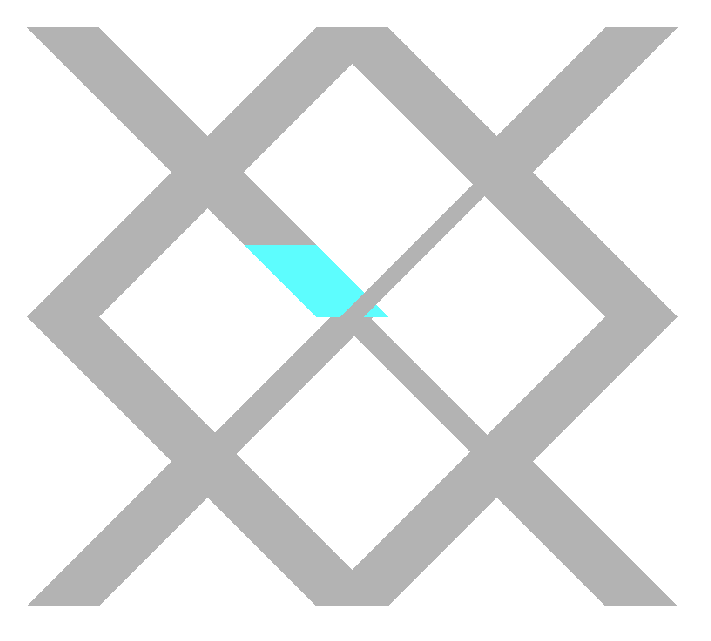
\includegraphics[width=8cm]{fig_test_dist_th01}
			\caption{Initial position of wetting fluid}
		\end{figure}

		\begin{figure}[H]
			\centering
			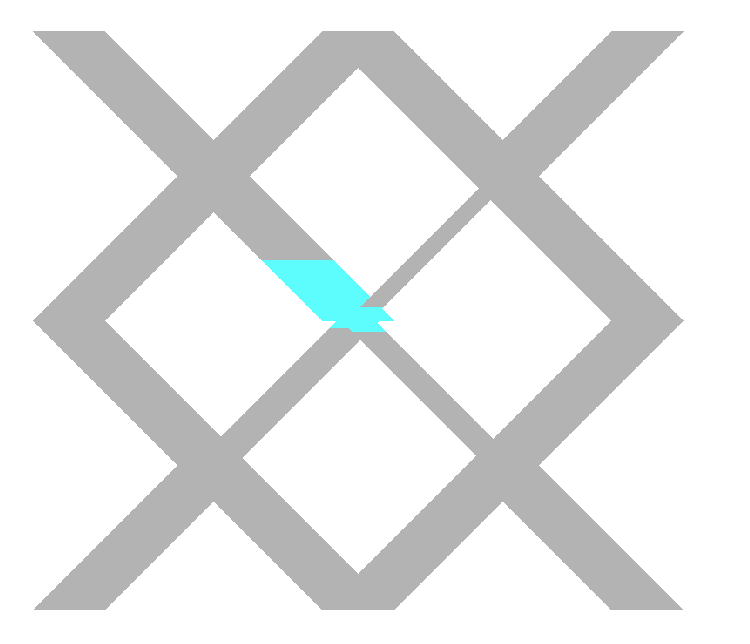
\includegraphics[width=8cm]{fig_test_dist_th02}
			\caption{The wetting fluid chose to move to the tubes with thinner radius.}
			
		\end{figure}
		
		\begin{figure}[H]
			\centering
			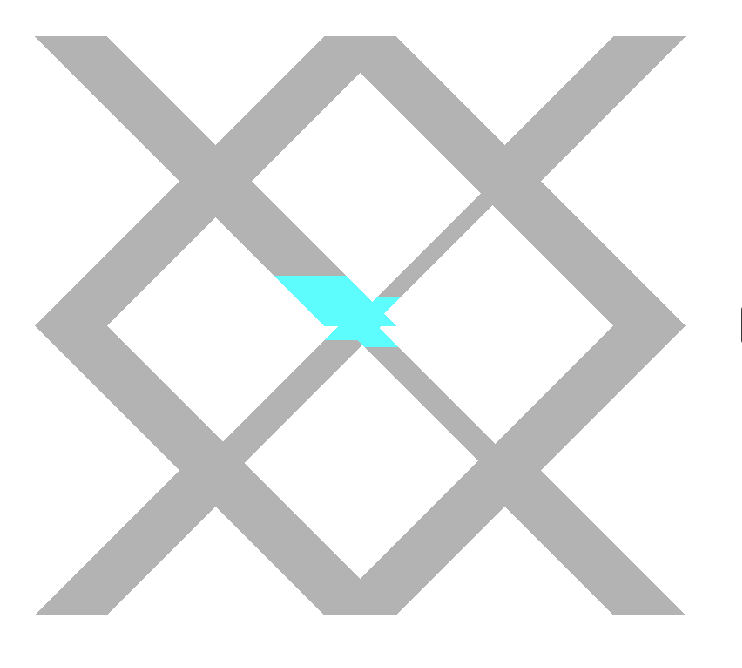
\includegraphics[width=8cm]{fig_test_dist_th03}
			\caption{The flow accelerates as more fluid is in the thinner radius, here viscosity of the wetting fluid is higher.}
		\end{figure}

		\begin{figure}[H]
			\centering
			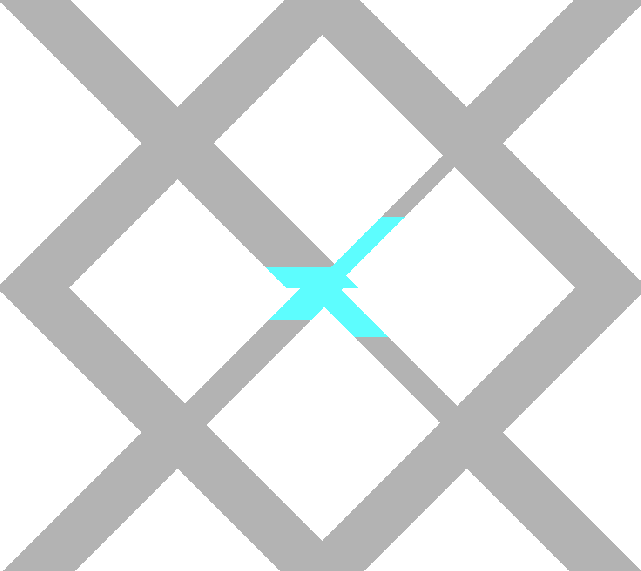
\includegraphics[width=8cm]{fig_test_dist_th04}
			\caption{}
		\end{figure}
		
		\begin{figure}[H]
			\centering
			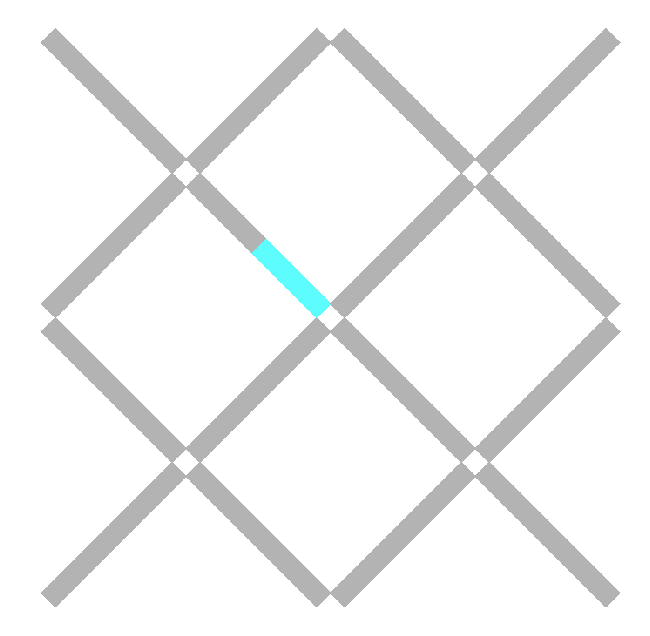
\includegraphics[width=8cm]{fig_test_dist_tn01}
			\caption{The same flow without plotting the radius thickness for clarity.}
		\end{figure}

		\begin{figure}[H]
			\centering
			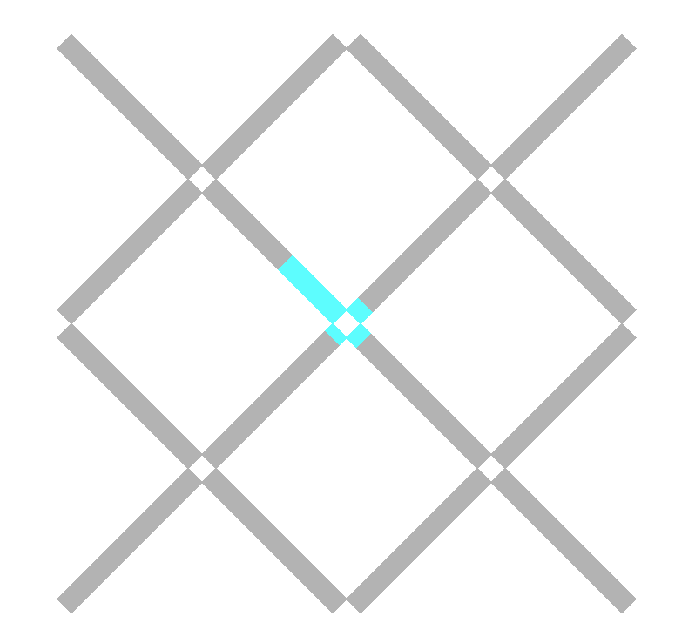
\includegraphics[width=8cm]{fig_test_dist_tn02}
			\caption{}
			
		\end{figure}
		
		\begin{figure}[H]
			\centering
			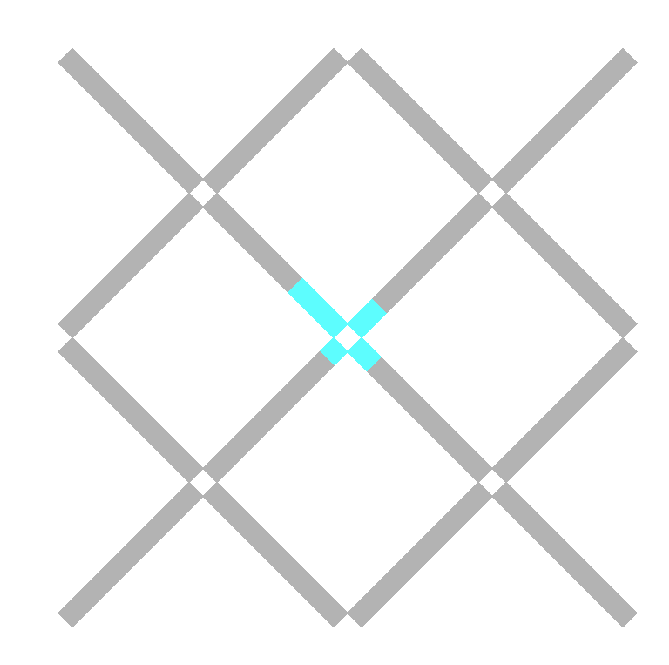
\includegraphics[width=8cm]{fig_test_dist_tn03}
			\caption{}
		\end{figure}

		\begin{figure}[H]
			\centering
			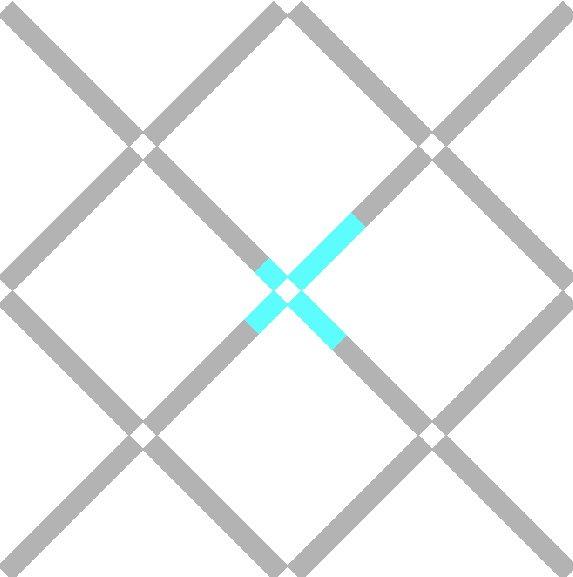
\includegraphics[width=8cm]{fig_test_dist_tn04}
			\caption{}
		\end{figure}
		
		
	\subsubsection{Displacement}
		\begin{figure}[H]
			\centering
			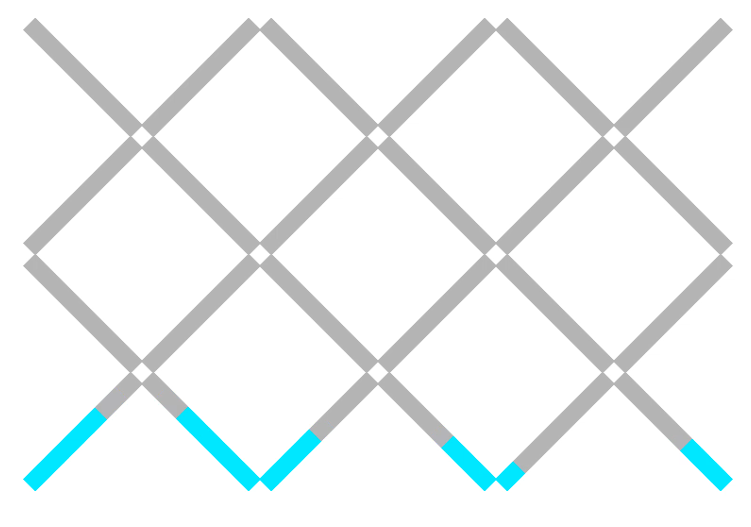
\includegraphics[width=8cm]{fig_initial-fill-distribution}
			\caption{Our model is initially set up such that the wetting fluid is low in saturation and is confined to the bottom of our network. A higher pressure is fixed for all nodes at the bottom layer, while a  low pressure is fixed for the top row.}
			\label{fig_plot-sat-vs-time-disp-one}
		\end{figure}

		\begin{figure}[H]
			\centering
			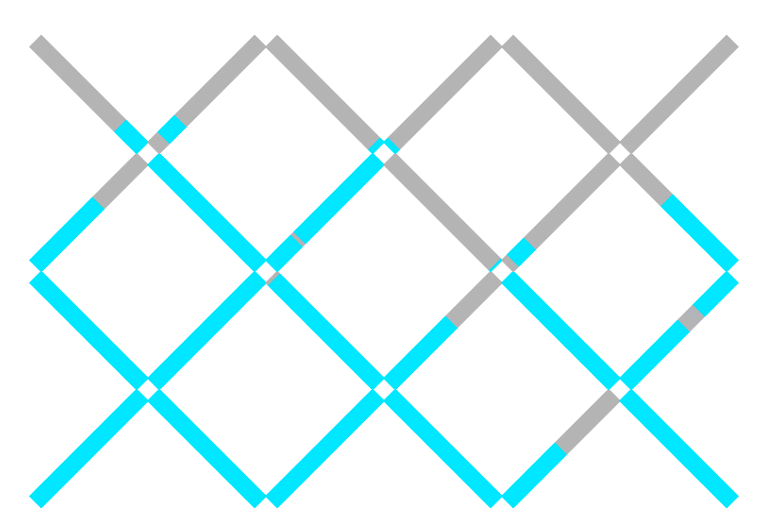
\includegraphics[width=8cm]{fig_final-fill-distribution}
			\caption{In all nodes, law of conservation of volume is applied, since mass is conserved and the phases are non-compressible. However for the bottom layer of nodes, the wetting fluid is injected as much required according to the sum of flow rates determined in the tubes connected to those nodes, while from the top layer of nodes a fluid is removed.}
			\label{fig_plot-sat-vs-time-disp-two}
		\end{figure}

\subsection{Initial conditions for the main experiment - imhibition}

	\begin{itemize}
		\item Closed boundaries.
		\item The aim of this simulation is observe the movement of wettable fluid (blue) from the region of thicker tube to the thinner tube.
		\item The saturation of each phase is measured in the region of thinner tubes.
		\item All boundaries are closed, the saturation of a phase for the whole system remains constant in time.
		\item The radius in the outer region is three times larger.
		\item The radius of the outer region is 3 times larger than inner.
		\item We plan to observe, that the invasion slows down and possibly oscillates, it is due to the meniscus in the inner region being ineffective to suck more blue fluid as most tubes have two meniscus. In our algorithm, tubes with two meniscus have a zero net pressure.
		\item EDIT Wetting(cyan) fluid into the region which contains thinner radius. The flow accelerates because, for a corner initially there are 3 meniscus, it multiplies into 3 when the meniscus reaches the node. The corner where the meniscus reaches the node late is pushed back because of the excessive pressures from the other corners.
	\end{itemize}
	
	\begin{figure}[H]
		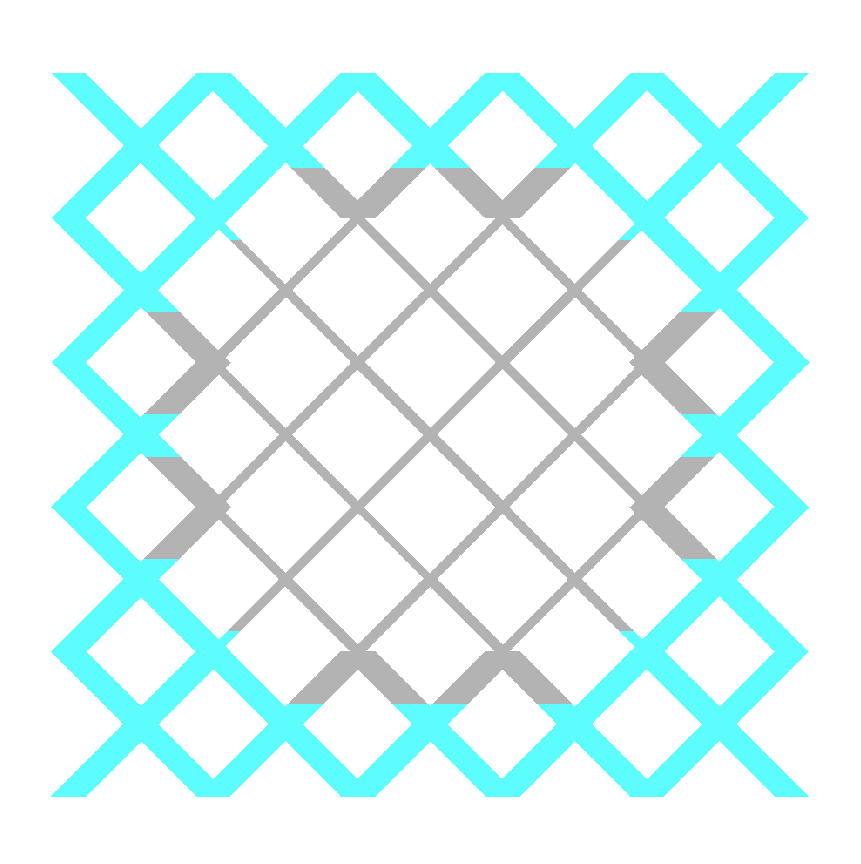
\includegraphics[height=8cm]{fig_result10by10_1}
		\caption{Initial setup, outer radius is 3 times larger than inner.}
		\label{fig_invasion-result1}
	\end{figure}	

	
\subsection{Linear equations in case of infinitely many solutions}
	It is possible to calculate the pressures at each node, if the pressures are known on the edges. However when we want to model imhibition, the boundaries are closed and the total volume of a phase remains the same.
	
	\begin{figure}[H]
		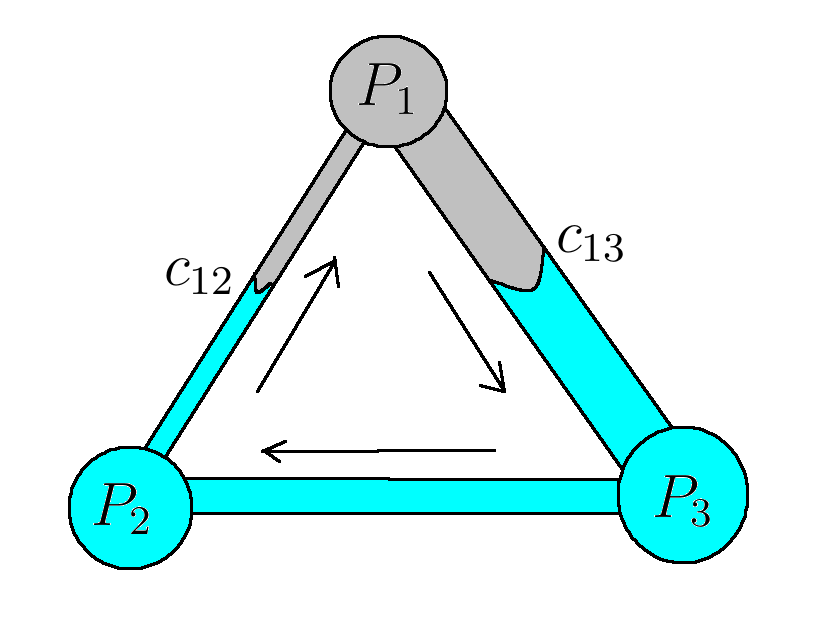
\includegraphics[height=6cm]{fig_zero-linearequation}
		\caption{Case of of infinitely many solutions}
	\end{figure}
	
	Let the flow rates be given by:
	\begin{equation}
		q_{ij} = k_{ij} \Delta P + c_{ij}
	\end{equation}
	
	For $N_{1}$:
	\[ q_{12} = k_{12}(P_1 - P_2) + c_{12} \]
	\[ q_{13} = k_{13}(P_1 - P_3) + c_{13} \]
	
	Since:
	\[ q_{12} + q_{13} = 0 \]
	\[(k_{12} + k_{13})P_1 - k_{12}P_2 - k_{13}P_3 = -c_{12} - c_{13} \]
	
	Then for each node we obtain the following matrix:
	
	\[ 
	\begin{pmatrix}
		(k_{12} + k_{13}) & -k_{12} & -k_{13} & -c_{12} - c_{13} \\
		-k_{21} & (k_{21} + k_{23}) & -k_{23} & -c_{21} - c_{23} \\
		-k_{31} & -k_{32} & (k_{31} + k_{32}) & -c_{31} - c_{32} \\
	\end{pmatrix}
	\]
	
	Note that:
	\[ k_{ij} = k_{ji} \]
	\[ c_{ij} = -c_{ji} \]
	
	Hence the sum of each column of this matrix is zero.
	
	By $R_3 = R_3 + R_1 + R_2$:
	
	\[ 
	\begin{pmatrix}
		(k_{12} + k_{13}) & -k_{12} & -k_{13} & -c_{12} - c_{13} \\
		-k_{21} & (k_{21} + k_{23}) & -k_{23} & -c_{21} - c_{23} \\
		0 & 0 & 0 & 0 \\
	\end{pmatrix}
	\]
	
	This is solved by adding a constant $a$ to one of the column of the matrix for each rows. In our model the centre was chosen to be the zero of pressure. Changing this point does not change the flow rates or the nature of flows.
	
	\[ 
	\begin{pmatrix}
		(k_{12} + k_{13}) & -k_{12} & -k_{13} + a & -c_{12} - c_{13} \\
		-k_{21} & (k_{21} + k_{23}) & -k_{23} + a & -c_{21} - c_{23} \\
		-k_{31} & -k_{32} & (k_{31} + k_{32}) + a & -c_{31} - c_{32} \\
	\end{pmatrix}
	\]
	
	After $R_3 = R_3 + R_1 + R_2$:
	\[ 
	\begin{pmatrix}
		(k_{12} + k_{13}) & -k_{12} & -k_{13} + a & -c_{12} - c_{13} \\
		-k_{21} & (k_{21} + k_{23}) & -k_{23} + a & -c_{21} - c_{23} \\
		0 & 0 & 3a & 0 \\
	\end{pmatrix}
	\]
	
	\[3aP_3 = 0 \]
	
	The solutions exists only if $P_3 = 0$.
	




 
	
